% !TEX root =  ../main.tex
\section{Gather}
\subsection{Definition}

\subsubsection{Signature} \cstr{gather(s : set<VM>)}

\begin{itemize}
\item \cstr{s} : a set of at least 2 VMs for a meaningful constraint. VMs not in the \st{Running} state are ignored.
\end{itemize}

The \cstr{gather} constraint forces all the running VMs in the set \cstr{s} to be hosted on the same server.

\classification{gather}{application administrator}{VM placement}{Performance,VM-to-VM placement}

\subsubsection{Usage}

The \cstr{gather} constraint may first be used by an application administrator to force the colocation of
 strongly communicating VMs.
Using one \cstr{gather} constraint, the VMs will be running on a same server and the virtual network between them will be embedded into the internal network provided by the hypervisor instead of the physical network, leading to better network performance.

The \cstr{gather} constraint may also be used by an application administrator to force the colocation
of VMs that have to share a component such as a filesystem. Without any guarantee of colocation, it is a necessary to rely on a distributed filesystem or a file server which provide less performance than a raw and direct access to the data. Using the colocation guarantee provided by a \cstr{gather} constraint, the filesystem
may be placed directly on the hosting server to achieve better performance. In this context, it is also often
desirable to use one \hyperref[cstr: root]{\cstr{root}} constraint to prevent from VMs relocation.

It has however to be noticed that these usages ask explicitly for the VMs colocation. It is then not allowed to host the VMs on several servers when the colocation is not possible. The application administrator should then  not over-estimate his needs to prevent him from having its VMs not running at all.

\subsubsection{Example}

Figure~\ref{fig: gather} depicts a sample reconfiguration between a source and a destination configuration. In this example, the following \cstr{gather} constraints were considered:

\begin{itemize}

\item \cstr{gather(\{VM1, VM4\})}. This constraint was satisfied in the source configuration as only \cstr{VM1}
was running, so considered in the constraint. The constraint is also satisfied in the destination configuration:
during the reconfiguration, \cstr{VM4} was set in the \st{Running} state and deployed on \cstr{N1} according to
the constraint requirement.

\item \cstr{gather(\{VM2, VM5\})}. This constraint was not satisfied in the source configuration as \cstr{VM4} and \cstr{VM5} were running on different servers. The reconfiguration fixed this violation by relocating \cstr{VM2} to \cstr{N3} which is also hosting \cstr{VM5}.

\item \cstr{gather(\{VM3, VM6\})}. This constraint was satisfied in the source configuration as both VMs were running on \cstr{N2}. Despite both VMs were relocated during the reconfiguration process, the constraint is still satisfied in the destination configuration as both VMs are running on \cstr{N4} and the end of reconfiguration.
\end{itemize}

\begin{reconfiguration}
\centering
\begin{minipage}[b]{0.40\textwidth}
\begin{lstlisting}
N1: VM1 VM2
N2: VM3 VM6
N3: VM5
N4: 
? : VM4
\end{lstlisting}
\end{minipage}
\begin{minipage}[b]{2cm}
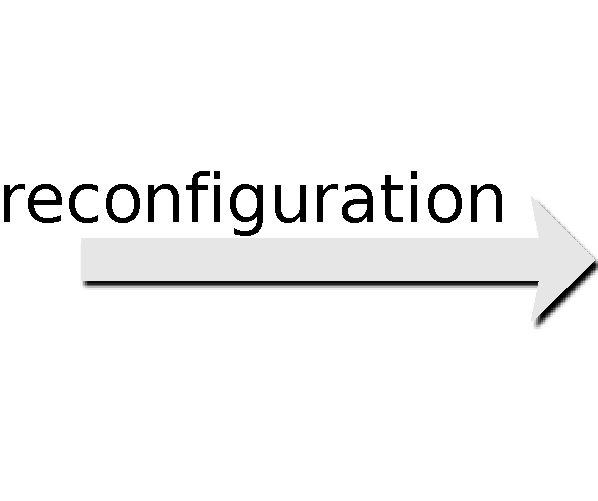
\includegraphics[width=2cm]{img/arrow_reconfiguration}
\end{minipage}
\begin{minipage}[b]{0.40\textwidth}
\begin{lstlisting}
N1: VM1 VM4
N2:
N3: VM5 VM2
N4: VM3 VM6
? :
\end{lstlisting}
\end{minipage}
\caption{A reconfiguration motivated by \cstr{gather} constraints.}\label{fig: gather}
\end{reconfiguration}

\fullVersion{
\subsection{Model}

The \cstr{gather} is modeled by forcing the d-slice placement variable associated to each running VM to be equal. In terms of RP variable, the constraint is modeled as follow:

\begin{equation*}
\begin{split}
\text{\cstr{gather(V : set<VM>)}}&\triangleq\\
&\forall v_i, v_j \in V, d_i^h = d_j^h
\end{split}
\end{equation*}

\subsection{Violation Detection}

The detection of the violating elements in \cstr{gather} consists in computing all the current hosting servers for the given running VMs. If there is only one server, then there is no misplaced VMs. Otherwise, there must be misplaced VMs. There is no safe solutions to detect the exact VMs that are misplaced within the scope of a \cstr{gather} constraint as each of the hosting server may be the \emph{right one}. It is however possible to count the minimal number of misplaced VMs. In practice, it is equals to the minimal number of involved VMs hosted on one of the servers.

\subsection{Availability}

\subsubsection{In {\btrp}}

This constraint is available in {\btrp} using the name \texttt{Gather}. Using the global constraint catalog~\cite{gccat}, the assignment of all the d-slice placement variables is ensure to be the same using \emph{eq} constraints. In practice, the \cstr{gather} constraint is modeled as follow:

\begin{equation*}
\begin{split}
\text{\cstr{gather(V : set<VM>)}}&\triangleq\\
   & \forall v_i,v_j \in V, eq(d_i^h, d_j^h)
\end{split}
\end{equation*}

\subsubsection{In VMWare}

Affinity rules between VMs allows to reproduce the \cstr{gather} constraint.
}
\subsection{See also}

\subsubsection{Related Constraints}
\begin{itemize}
\item \cstrref{spread}, \cstrref{lazySpread}: the opposite constraints of \cstr{gather} that force the VMs to be hosted on distinct servers.
\end{itemize}

\emulatedWith{gather}{among}{\cstr{gather(s)}}{\cstr{among(s,\allNodes/|\allNodes|)}}
\printListOfInheritance{gather}